% !TEX TS-program = xelatex
%
% Created by Gerson Sunyé on 2016-12-14.
% Copyright (c) 2016 .
\documentclass[a4paper,11pt]{memoir}
\usepackage[utf8]{inputenc}
\usepackage{lmodern}
\usepackage{listings,multicol}
\usepackage{hyperref}
\usepackage{graphicx}
\usepackage[svgnames]{xcolor}
\usepackage{polyglossia}
\setdefaultlanguage{english}
\usepackage{pdfpages}
\usepackage{typehtml}
\usepackage{lscape}
\usepackage[french,boxed,lined]{algorithm2e}
\usepackage{amsmath}
\usepackage{siunitx}
\usepackage{exsheets}
\SetupExSheets{solution/print=true}
\usepackage{booktabs}
\usepackage{paralist}


\lstset{basicstyle=\footnotesize,
	tabsize=3,
	keywordstyle=\bfseries,
	stringstyle=\ttfamily,
	showstringspaces=\false,
	frame=tb,
	commentstyle=\itshape\color{magenta},
	%extendedchars=\true,
	numbers=left, 
	numberstyle=\tiny,
	sensitive,
	texcl,
	breaklines=true,
	literate={é}{e}{1} {à}{a}{1}
	}

\lstnewenvironment{java}{\lstset{language=Java,        
        flexiblecolumns,
        sensitive, 
		texcl
        }}{}
		
\newcommand{\code}[1]{\lstinline{#1}} 
\graphicspath{{./img/}}

\chapterstyle{ell}


% \firstpageheader{Test logiciel}{Exercices}{Page \thepage\ of \numpages}
% \firstpageheadrule

\title{{\Huge\bfseries Software Construction and Evolution} \\[5pt] {\Large\bfseries Instructor-led Exercices}}
\date{}
\author{Gerson Sunyé \\ \href{mailto:gerson.sunye@univ-nantes.fr}{gerson.sunye@univ-nantes.fr} \\ Université de Nantes
\and Gilles Ardourel \\ \href{matilto:gilles.ardourel@univ-nantes.fr}{gilles.ardourel@univ-nantes.fr} \\ Université de Nantes
}

\newcommand*{\plogo}{\fbox{$\mathcal{PL}$}} % Generic publisher logo
\newcommand*{\rotrt}[1]{\rotatebox{90}{#1}} % Command to rotate right 90 degrees
\newcommand*{\rotlft}[1]{\rotatebox{-90}{#1}} % Command to rotate left 90 degrees
\newcommand*{\titleBC}{\begingroup % Create the command for including the title page in the document
\centering % Center all text

\def\CP{\textit{\Huge Software Construction and Evolution}} % Title

\settowidth{\unitlength}{\CP} % Set the width of the curly brackets to the width of the title
{\color{LightGoldenrod}\resizebox*{\unitlength}{\baselineskip}{\rotrt{$\}$}}} \\[\baselineskip] % Print top curly bracket
\textcolor{Sienna}{\CP} \\[\baselineskip] % Print title
{\color{RosyBrown}\Large Instructor-led Exercices} \\ % Tagline or further description
{\color{LightGoldenrod}\resizebox*{\unitlength}{\baselineskip}{\rotlft{$\}$}}} % Print bottom curly bracket

\vfill % Whitespace between the title and the author name

%{\textbf{John Smith}}\\ % Author name

{\Large \textbf{Gerson Sunyé} \\ \href{mailto:gerson.sunye@univ-nantes.fr}{gerson.sunye@univ-nantes.fr} \\ Université de Nantes} \\[10pt]
{\Large \textbf{Gilles Ardourel} \\ \href{matilto:gilles.ardourel@univ-nantes.fr}{gilles.ardourel@univ-nantes.fr} \\ Université de Nantes} \\[10pt]


\vfill % Whitespace between the author name and the publisher logo

\plogo\\[0.5\baselineskip] % Publisher logo
2017 % Year published

\endgroup}



\begin{document}
%\maketitle
\titleBC

% \begin{center}
%   \fbox{\parbox{0.9\textwidth}{\centering
%         Answer the questions in the spaces provided on the
%         question sheets. If you run out of room for an answer,
%         continue on the back of the page.}}
% \end{center}

% \vspace{0.5cm}
% \makebox[0.9\textwidth]{Name:\enspace\hrulefill}


%\begin{questions}
	
\chapter{Mapping UML Designs to Code}


During Software Construction, the mapping between design models and source code is essential. 
Use the concepts introduced during the lectures to propose the implementation of the design models below.

\begin{question}\textbf{Type Correspondence}

\begin{inparaenum}[(A)]
	\item First, complete Table~\ref{tab:monovalued} to propose a correspondence between UML and Java types for mono-valued attributes.
	\item Second, complete Table~\ref{tab:multivalued}, to propose a similar correspondence table, but for multi-valued attributes. Use the classes and interfaces provided by the Java Collection Framework (JCF).
\end{inparaenum}

\begin{table}
	\begin{center}
		\begin{tabular}{p{5cm}p{5cm}}
			\toprule
			\textbf{UML} & \textbf{Java}\\
			\midrule
String   & \\
Integer  & \\
Real 	  & \\
Boolean  & \\
UnlimitedNatural & \\
			\bottomrule
		\end{tabular}
	\end{center}
	\caption{Types for mono-valued attributes}
	\label{tab:monovalued}
\end{table}



\begin{table}
	\begin{center}
		\begin{tabular}{p{7cm}p{5cm}}
			\toprule
			\textbf{UML} & \textbf{Java}\\
			\midrule
			             \emph{AnyType} [*] \{unique, ordered\}  & \\
			              \emph{AnyType} [*] \{unique, unordered\}   & \\
			              \emph{AnyType} [*] \{nonunique, ordered\}  	  & \\
						  \emph{AnyType} [*] \{nonunique, unordered\}   & \\
			\bottomrule
		\end{tabular}
			\end{center}
			\caption{Types for multi-valued attributes}
			\label{tab:multivalued}
		\end{table}
\end{question}




\begin{question}
	\textbf{Attribute Implementation (Getter/Setter approach)} 
	
Use Java to implement the class \code{Event} and its attributes. 
Use the Getter/Setter implementation strategy introduced during the lectures.  


\begin{figure}[htbp]
	\centering
		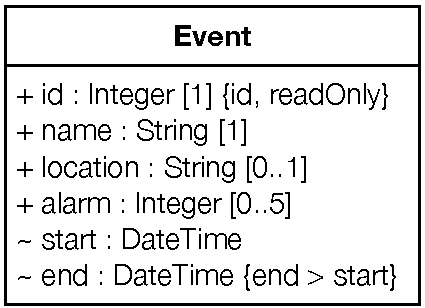
\includegraphics[width=.4\linewidth]{CD-Event.pdf}
	\caption{The Event Class}
	\label{fig:event}
\end{figure}	

\begin{inparaenum}[(A)]
	\item First, declare the Java class and its fields.
	\item Now, declare the class constructor. Remember that some attributes are mandatory and others are not.
	\item Finally, declare the fields' accessors and modifiers (getters and setters). Remember to respect the attribute visibility.
	\item Now, decide how to deal with errors, for instance a start date that is later than the end date. 
\end{inparaenum}
\end{question}

\begin{solution}
			There are several ways to deal with errors in Java. In my solution I used assertions, which is a simple solution, but not adapted to public methods. Using runtime exceptions, such as \code{IllegalArgumentException} for the dates and \code{IndexOutOfBoundsException} for multivalued attributes is a more ``java-oriented'' approach. Another interesting approach is the use of AssertJ, which helps developers to specify simple and elegant assertions. Guava, Apache commons, and Lombok are also interesting alternatives to validate parameters.
			
			Alternatives: create our own exceptions, use normal exceptions (not Runtime). Use integers (c-oriented approach.)
%\lstset{language=Java}

\lstinputlisting[language=Java]{./src/main/java/fr/unantes/event/Event.java}

\end{solution}
	
	
\begin{question}
	\textbf{Attribute Implementation (Wrapper approach)}
	
Now, use the Wrapper implementation strategy introduced during the lectures to implement the Event class.
	\begin{inparaenum}
		\item For dealing with the multi-valued attribute \code{alarm}, define a wrapper class that is able to check its multiplicity.
		\item Do the same for the mono-valued attributes. Use Java generic types.
	\end{inparaenum}
\end{question}
\begin{solution}
	\lstinputlisting[language=Java]{./src/main/java/fr/unantes/event/Event.java}
	\lstinputlisting[language=Java]{./src/main/java/fr/unantes/event/MonovaluedAttribute.java}
	\lstinputlisting[language=Java]{./src/main/java/fr/unantes/event/ReadOnlyMonovaluedAttribute.java}
	\lstinputlisting[language=Java]{./src/main/java/fr/unantes/event/MultivaluedAttribute.java}
\end{solution}


\begin{question}
	\textbf{Unidirectional Association Implementation}

Figures~\ref{fig:unidirectional} and~\ref{fig:unique} present two different versions of a unidirectional association between the classes \code{Window} and \code{Field}.
Use Java to implement the classes \code{Window} and \code{Field}, as well as the association between both.

\begin{figure}[htbp]
	\centering
	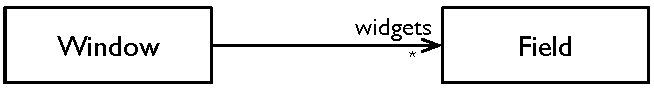
\includegraphics[scale=.8]{CD-WindowFieldUni.pdf}
	\caption{Unidirectional Association}
	\label{fig:unidirectional}
\end{figure}

\begin{figure}[htbp]
	\centering
		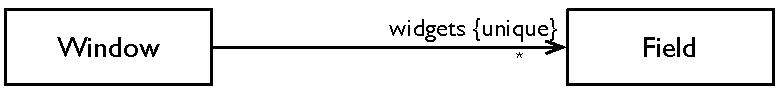
\includegraphics[scale=.8]{CD-WindowFieldUnique.pdf}
	\caption{Unidirectional Unique Association}
	\label{fig:unique}
\end{figure}



\begin{inparaenum}[(A)]
	\item First, for dealing with unidirectional multivalued association roles, define a generic class named \code{Reference} that could be reused by other implementations.
	\item Make your class flexible enough to handle unique et non unique association roles.
	\item Then, declare the Java classes and its fields.
\end{inparaenum}

\end{question}

\begin{solution}
		\lstset{language=Java}
		\lstinputlisting{./src/main/java/fr/unantes/unidirectional/Window.java}
		\lstinputlisting{./src/main/java/fr/unantes/unidirectional/Field.java}	
\end{solution}



\begin{question}
	\textbf{Bidirectional Association Implementation}

The UML class model presented in Figures~\ref{fig:readOnly} and~\ref{fig:bidirectional}
are similar to the previous ones, except that the association between both classes are bidirectional.

Use Java to implement the classes \code{Window} and \code{Field}, as well as the association between both.
Remember that you must handle the handshake problem.

\begin{figure}[htbp]
	\centering
		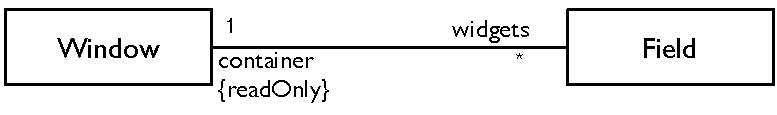
\includegraphics[scale=.8]{CD-WindowFieldReadOnly.pdf}
	\caption{Bidirectional Read-Only Association}
	\label{fig:readOnly}
\end{figure}

\begin{figure}[htbp]
	\centering
		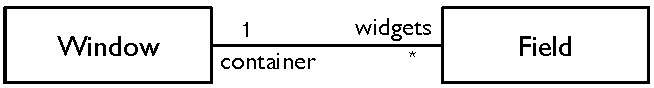
\includegraphics[scale=.8]{CD-WindowField.pdf}
	\caption{Bidirectional Association}
	\label{fig:bidirectional}
\end{figure}	


\begin{inparaenum}[(A)]
	\item First, define a class named \code{ReferenceToWindow} that will handle the mono-valued association role \code{container}, from \code{Field} to \code{Window}. This class must implement the methods \code{get()}, \code{set()}, and \code{unset}.
	\item Then, define a class named \code{ReferenceToField} that will handle the multivalued association role \code{widgets}, from \code{Window} to \code{Field}. This class must implement the methods \code{add()}, \code{remove()}, and \code{contains()}.
	\item Now, add the code needed to handle the handshake. 
	\item Finally, declare the Java classes \code{Window} and \code {Field}, and their fields.
\end{inparaenum}
	
\end{question}

\begin{solution}
		\lstset{language=Java}
		\lstinputlisting{./src/main/java/fr/unantes/bidirectional/Window.java}
		\lstinputlisting{./src/main/java/fr/unantes/bidirectional/Field.java}	
\end{solution}

\begin{question}
	\textbf{Wrapping Things Up}
	
	Use Java to implement the diagram depicted by Figure~\ref{fig:team}.

	\begin{figure}[htbp]
		\centering
			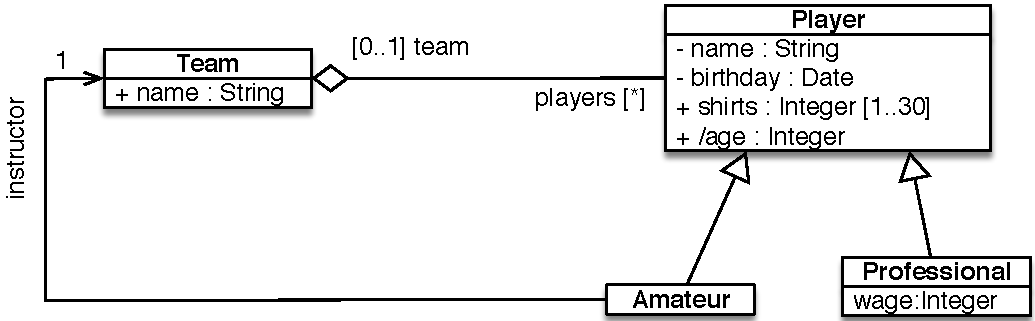
\includegraphics[width=.8\linewidth]{Team}
		\caption{UML Class Diagram\--- Team}
		\label{fig:team}
	\end{figure}
	
\end{question}


\end{document}


